\documentclass{article}
\usepackage{graphicx} % Required for inserting images
\usepackage{mdframed}
\usepackage{setspace}
\usepackage{multirow}
\usepackage{multicol}
\usepackage{hyperref}
\usepackage{xcolor}


% to adjust line spacing for lists
\usepackage{enumitem}

% Font 
\usepackage{lipsum}
\usepackage{cmbright}

\usepackage{geometry}
\geometry{left=2cm, right=2cm, bottom=3cm, top=3cm}

\usepackage{float}
\usepackage{listings}
\usepackage{amsthm}
\usepackage{amsmath}
\usepackage{amssymb}
\usepackage{tikz}
\usepackage[table,xcdraw]{xcolor} % for \rowcolor and colored rules
\usepackage{tabularx}             % for tabularx environment
\usepackage{array}                % for custom column widths and formatting


%Colors
\definecolor{peach}{RGB}{255, 190, 170}
\definecolor{yellow}{RGB}{252, 239, 145}
\definecolor{codegreen}{rgb}{0,0.6,0}
\definecolor{codegray}{rgb}{0.5,0.5,0.5}
\definecolor{codepurple}{rgb}{0.58,0,0.82}
\definecolor{backcolour}{rgb}{0.95,0.95,0.92}
\definecolor{lightblue}{RGB}{220, 233, 252}
\definecolor{blue}{RGB}{0, 119, 182}
\definecolor{lightgreen}{RGB}{220, 255, 240}
\definecolor{darkgreen}{RGB}{0, 100, 0}
\definecolor{bordergreen}{RGB}{0, 128, 0}


\definecolor{peach}{RGB}{255, 190, 170}
\definecolor{yellow}{RGB}{252, 239, 145}
\definecolor{codegreen}{rgb}{0,0.6,0}
\definecolor{codegray}{rgb}{0.5,0.5,0.5}
\definecolor{codepurple}{rgb}{0.58,0,0.82}
\definecolor{backcolour}{rgb}{0.95,0.95,0.92}

\definecolor{lightblue}{RGB}{220, 233, 252}
\definecolor{blue}{RGB}{0, 119, 182}
\definecolor{lightgreen}{RGB}{220, 255, 240}
\renewcommand{\contentsname}{CONTENT}

% Stilimi per kodin
\lstdefinestyle{mystyle}{
    backgroundcolor=\color{lightblue},   
    commentstyle=\color{codegreen},
    keywordstyle=\color{magenta},
    numberstyle=\tiny\color{codegray},
    stringstyle=\color{codepurple},
    basicstyle=\ttfamily\footnotesize,
    breakatwhitespace=false,         
    breaklines=true,                 
    captionpos=b,                    
    keepspaces=true,                 
    numbers=left,                    
    numbersep=5pt,                  
    showspaces=false,                
    showstringspaces=false,
    showtabs=false,                  
    tabsize=2
}
\lstset{style=mystyle}

\usepackage{tcolorbox}
\newtcbox{\codebox}{on line, box align=base, colback=lightblue, colframe=white,
    boxsep=0.5pt, left=2pt, right=2pt, top=1pt, bottom=1pt}

\usepackage{tabularx}
\usepackage{array}
\usepackage{lstmisc}

\begin{document}

\clearpage
\thispagestyle{empty}

\begin{normalsize}
    \begin{center}
        \textbf{UNIVERSITETI I PRISHTINËS “HASAN PRISHTINA” \\
        FAKULTETI I SHKENCAVE MATEMATIKO-NATYRORE\\
        DEPARTAMENT OF MATHEMATICS, COMPUTER SCIENCE PROGRAM}
      \vspace{0.5in}
        
        \begin{figure}[h]
             \center
            
\includegraphics[scale=0.4]{images/up_logo.png}
        \end{figure}
        \vspace{0.5in}
        
        \Large{\textbf{Machine Learning \\ Seminar Project\\ Data Analysis for Diabetes Prediction Using Health Indicators}}
    \end{center}
\vspace{1in}

\setlength{\parindent}{7cm}

\begin{center}
    \textbf{Albana Rexhepi, Eljesa Kqiku, Kaltrina Kuka}\\ 
    \vspace{0.2cm}
  \textbf{May 2025}  
\end{center}
\end{normalsize}
\newpage
\tableofcontents
\newpage
\section{Introduction}
\subsection{Dataset description}
This dataset contains detailed health indicators collected from a large population and is designed to support the analysis and prediction of diabetes risk. It includes a variety of columns describing lifestyle factors and demographic data, such as high blood pressure (HighBP), high cholesterol (HighChol), body mass index (BMI), smoking and alcohol use, physical activity, diet, mental and physical health status, as well as gender, age, education level, and income.

The main variable of interest is Diabetes\_binary, which indicates whether an individual has been diagnosed with diabetes (1) or not (0). This dataset can be used to develop classification models aimed at predicting diabetes risk based on known behavioral and health-related factors.

\begin{table}[ht]
\centering
\begin{tabular}{|l|l|l|}
\hline
index & feature & description \\
\hline
Diabetes\_binary & 0 = no diabetes, 1 = diabetes & Diabetes status \\
\hline
HighBP & 0 = no high BP, 1 = high BP & High blood pressure \\
\hline
HighChol & 0 = no high cholesterol, 1 = high cholesterol & High cholesterol \\
\hline
CholCheck & 0 = no cholesterol check in 5 years, 1 = yes & Cholesterol check \\
\hline
BMI & Continuous & Body Mass Index \\
\hline
Smoker & 0 = no, 1 = yes & Smoked at least 100 cigarettes in life \\
\hline
Stroke & 0 = no, 1 = yes & Ever had a stroke \\
\hline
HeartDiseaseorAttack & 0 = no, 1 = yes & Heart disease or heart attack history \\
\hline
PhysActivity & 0 = no, 1 = yes & Physical activity in past 30 days (not job-related) \\
\hline
Fruits & 0 = no, 1 = yes & Consumes fruit 1+ times per day \\
\hline
Veggies & 0 = no, 1 = yes & Consumes vegetables 1+ times per day \\
\hline
HvyAlcoholConsump & 0 = no, 1 = yes & Heavy alcohol consumption \\
\hline
AnyHealthcare & 0 = no, 1 = yes & Healthcare coverage \\
\hline
NoDocbcCost & 0 = no, 1 = yes & Couldn’t see a doctor due to cost \\
\hline
GenHlth & 1 = excellent, 5 = poor & General health status \\
\hline
MentHlth & 1-30 days & Poor mental health days in the past 30 days \\
\hline
PhysHlth & 1-30 days & Physical illness/injury days in past 30 days \\
\hline
DiffWalk & 0 = no, 1 = yes & Difficulty walking or climbing stairs \\
\hline
Sex & 0 = female, 1 = male & Gender \\
\hline
Age & 1 = 18-24, 9 = 60-64, 13 = 80 or older & Age category \\
\hline
Education & 1-6 & Education level \\
\hline
Income & 1-8 & Income scale \\
\hline
\end{tabular}
\caption{List of all attributes in the dataset}
\end{table}


\subsection{Motivation of the study}

The motivation of this study is based on three main questions related to understanding the risk factors for diabetes and how these factors can be used to predict the likelihood of developing the disease:

\begin{enumerate}
    \item \textbf{What are the main factors that predict the risk of diabetes?} One objective of this study is to identify the health and lifestyle factors most strongly associated with the risk of developing diabetes. These factors, such as \texttt{BMI}, \texttt{Age}, and \texttt{Physical\_Health}, can help in early detection and prevention of diabetes.
    
    \item \textbf{Can a subset of factors be used to accurately predict whether an individual has diabetes?} Another important question is whether only a few factors, such as \texttt{BMI} and \texttt{Age}, can be used to make an accurate prediction of diabetes, simplifying the prediction process without losing too much accuracy.
    
    \item \textbf{How can machine learning models be used to predict diabetes risk more accurately?} This broader question relates to using advanced techniques to help create a reliable model for predicting diabetes. Machine learning can uncover relationships and patterns that may not be immediately apparent using traditional methods.
\end{enumerate}

Through these questions, the study aims to improve our understanding of the factors influencing diabetes risk and to develop a simple yet accurate method for predicting who may be at risk.


\subsection{Selection of algorithms for the dataset}

For this dataset, where the target variable is \texttt{Diabetes\_binary} (diabetes status), three well-known machine learning algorithms have been chosen: \textbf{MLP (Multilayer Perceptron)}, \textbf{Autoencoder}, and \textbf{I TRETI}. These algorithms are suitable for this type of problem for various reasons:

\begin{itemize}
    \item \textbf{MLP (Multilayer Perceptron)}: \\
    MLP is a type of neural network that uses multiple processing layers and is excellent for handling classification and regression problems. This algorithm is powerful for capturing complex relationships between different features. For our dataset, it is well-suited to model the connections between health indicators and diabetes risk, as it can effectively analyze factors such as \texttt{BMI}, \texttt{Age}, \texttt{Physical\_Health}, \texttt{Smoking}, and other related variables.

    \item \textbf{Autoencoder}: \\
    An Autoencoder is a type of neural network used primarily for unsupervised learning and dimensionality reduction. It can help identify hidden patterns in the data and is useful for reducing the number of features while maintaining the underlying structure. For our dataset, it can assist in detecting underlying factors contributing to diabetes risk by learning an efficient representation of the data. Autoencoders are also useful for feature extraction, especially in cases where the data is high-dimensional.
    
    \item \textbf{[Third Algorithm]}: \\
    flasum per tretin
\end{itemize}

\section{Preprocessing}

At this part of the project, we begin with the data preprocessing phase. This step is necessary to prepare the dataset for machine learning, ensuring the data is ready for analysis and modeling.

\subsection{Data cleaning}
\subsubsection{Removing Duplicates}
For this step, we first analyze if there are any duplicate rows in the dataset using the following Python code:

\lstinputlisting[language=python]{../code/duplicate_remover.py}


After running the code, we found that there are 1635 duplicate rows. However, since these duplicates could potentially represent individuals who share the same health indicators (such as age, BMI, or smoking status), and not necessarily represent data entry errors, we decided not to remove them. This is because, in medical datasets, it is common for multiple individuals to have identical data points across various features. Therefore, removing these rows could lead to loss of valid data.

\begin{lstlisting}[language=bash]
Found 1635 duplicate rows.
\end{lstlisting}

As shown, there are 1635 duplicate rows, but they are not removed to ensure we preserve all relevant data for analysis.

\subsubsection{Handling missing values}

In this step, we aim to check whether the dataset contains any missing values. Missing data can impact the accuracy of machine learning models, so identifying and addressing it is an important part of the data preprocessing process. Below is the Python code used for this task:

\lstinputlisting[language=python]{../code/missing_values.py}

The output after executing the script was:

\begin{lstlisting}[language=bash]
Diabetes_binary         0
HighBP                  0
HighChol                0
CholCheck               0
BMI                     0
Smoker                  0
Stroke                  0
HeartDiseaseorAttack    0
PhysActivity            0
Fruits                  0
Veggies                 0
HvyAlcoholConsump       0
AnyHealthcare           0
NoDocbcCost             0
GenHlth                 0
MentHlth                0
PhysHlth                0
DiffWalk                0
Sex                     0
Age                     0
Education               0
Income                  0
\end{lstlisting}

As we can see, all columns in the dataset have a count of 0 missing values. This means the dataset is complete in terms of data presence, and no additional cleaning or imputation for missing values is necessary.

\subsection{Data integration}
In this project, all the required data is already combined into a single CSV file. Therefore, no additional integration from multiple sources is necessary. The dataset is self-contained and ready for the next steps of data preprocessing.

\subsection{Data transformation}

In this step, we apply feature scaling to the dataset in order to standardize the features. Scaling is necessary because some machine learning algorithms, such as the ones we have chosen for this analysis, are sensitive to the scale of the data. These algorithms work better when all features have a similar range.

\subsubsection{Handling outliers}

The first step we used to analyze the outlier or noise values was checking the min, max, average and mode of each attribute. From these data we can conclude that there are no noises since all the min-max fields are within the range declared on the metadata.
\noindent Next we tried finding any outlier with the interquartile range, but this method didn't give

\lstinputlisting[language=python]{../code/outliers_handler.py}

\subsubsection{Data scaling}

In this step, we apply feature scaling to the dataset in order to standardize the features. Scaling ensures that all features have a similar range. The StandardScaler from the \texttt{sklearn.preprocessing} library is used to perform scaling.

The following Python code demonstrates the process of scaling the features of the dataset:

\lstinputlisting[language=python]{../code/scaling.py}


This code scales all the features of the dataset using the \texttt{StandardScaler}, which standardizes the features by removing the mean and scaling to unit variance. The scaled features are then saved in a new CSV file called \texttt{diabetes\_scaled.csv}. 

\section{Prepare for analysis}

\subsection{Correlation between features}

Understanding how features interact within the dataset is a key step before building predictive models. One effective way to explore these interactions is through correlation analysis. This technique reveals the strength and direction of linear relationships between variables, helping us detect redundant features, highlight those most relevant to the target variable, and optimize the feature set for better model efficiency and accuracy. By refining the input space early on, we set a strong foundation for the performance of our machine learning models.

One important aspect of correlation analysis is examining how strongly each feature relates to the target variable, in this case, Diabetes\_binary. Identifying variables that show a higher correlation with the target can guide us in selecting the most predictive features for our model. On the other hand, features that exhibit very weak relationships with the target may contribute little to the predictive power and can be excluded to simplify the model. Additionally, correlation analysis helps reveal whether certain features are highly related to each other. When two features show a strong correlation such as above 0.5 it may indicate redundancy. Retaining both could introduce multicollinearity, which not only complicates model interpretation but can also impair the algorithm’s performance. In such cases, it's often beneficial to remove one of the correlated features to streamline the dataset and enhance model robustness.

To calculate the correlation between features, we used the \texttt{corr()} function from the \texttt{pandas} library.  
We visualized the results using a Heatmap. A heatmap is a graphical representation that uses color gradients to indicate the strength of relationships in a two-dimensional matrix. This is especially useful for identifying patterns and connections between features.

The implementation can be seen in the code below, and the visual results are presented in Figure \ref{fig:correlation-matrix}:

\lstinputlisting[language=python]{../code/correlation.py}

\begin{figure}[H]
    \centering
oo    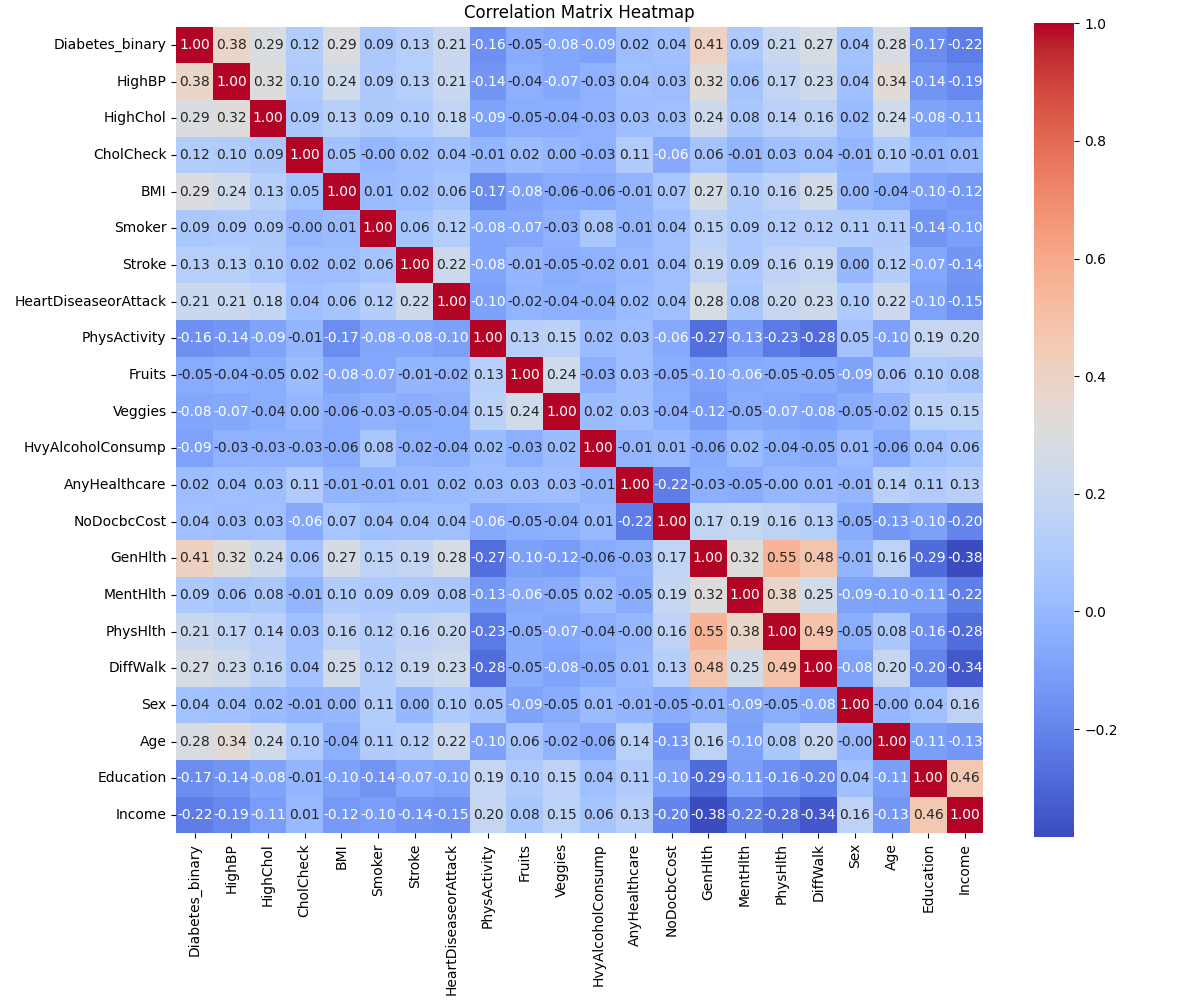
\includegraphics[width=0.7\textwidth]{images/diabetes_correlation_matrix.png}
    \caption{Correlation matrix between features.}
    \label{fig:correlation-matrix}
\end{figure}

From the heatmap visualization, we observe that some features are more strongly correlated with each other. We then filtered the feature pairs that have an absolute correlation higher than 0.45. The implementation of this filtering process in Python is shown below:

\lstinputlisting[language=python]{../code/correlation_filter.py}

The results are displayed in Table \ref{table:correlation-filtered}:

\begin{table}[ht]
\centering
\begin{tabular}{ |l|l|r| }
\hline
% \rowcolor{gray!30}
\textbf{Feature 1} & \textbf{Feature 2} & \textbf{Correlation} \\
\hline
GenHlth    & PhysHlth   & 0.552757 \\
PhysHlth   & DiffWalk   & 0.487976 \\
GenHlth    & DiffWalk   & 0.476639 \\
Education  & Income     & 0.460565 \\
\hline
\end{tabular}
\caption{Feature pairs with correlation $c > |0.45|$}
\label{table:correlation-filtered}
\end{table}
\subsection{hej}
To address weak correlation with the target variable, we will remove features exhibiting an absolute Pearson correlation coefficient of less than 0.1 with the 'Diabetes_binary' column. This step aims to eliminate features with a minimal linear relationship to the outcome we are trying to predict, potentially reducing noise and simplifying the model.

Subsequently, to mitigate the issue of multicollinearity among the remaining features, we will identify pairs of features with a high absolute Pearson correlation coefficient (greater than 0.45). For each such pair, one of the features will be removed. The decision on which feature to remove will be based on its correlation with the target variable; the feature with the weaker absolute correlation to 'Diabetes_binary' will be prioritized for removal. This strategy aims to reduce redundancy in the feature set, which can lead to instability and interpretability issues in some models, without significantly sacrificing predictive power related to the target.

\section{Algorithm implementation}
Next, we will implement the three chosen algorithms: MLP (Multilayer Perceptron), Autoencoder, and [Third Algorithm]. These algorithms have been selected due to their suitability for classification problems and their ability to handle structured and complex datasets. First, we will provide a brief introduction to each algorithm, highlighting their key characteristics. After that, we will proceed with the implementation and performance analysis for our dataset.

\subsection{Multilayer Perceptron (MLP)}

The \textbf{Multilayer Perceptron (MLP)} is a core model in the field of machine learning, used for both classification and regression tasks. MLP consists of three primary layers: the \textbf{input layer}, one or more \textbf{hidden layers}, and the \textbf{output layer}. Each layer contains multiple neurons, and neurons from one layer are fully connected to neurons in the next layer. This dense connectivity allows MLP to capture complex relationships in data, particularly non-linear ones, which are common in many real-world applications \cite{deeplearning1}.

In the context of our dataset, which includes health-related features such as \texttt{BMI}, \texttt{Age}, \texttt{Physical\_Health}, and \texttt{Sleep\_Time}, MLP is well-suited to identify hidden patterns and make predictions about whether an individual has diabetes or not. The network learns from the data through a process called \textit{backpropagation}, where errors from the output are propagated back through the network to adjust the weights of the connections between neurons. This process is combined with \textit{gradient descent}, an optimization technique that minimizes the prediction error by adjusting the weights during each iteration of training. Over time, the model learns the optimal weights, improving its ability to make accurate predictions \cite{nn1}.

The basic structure of an MLP is illustrated in the figure below. The input features, such as \texttt{BMI} and \texttt{Age}, are fed into the input layer. From there, they pass through one or more hidden layers, where neurons transform the data by applying learned weights and activation functions. The transformed data then flows to the output layer, which produces the final prediction, such as whether an individual has diabetes.

\begin{figure}[H]
    \centering
    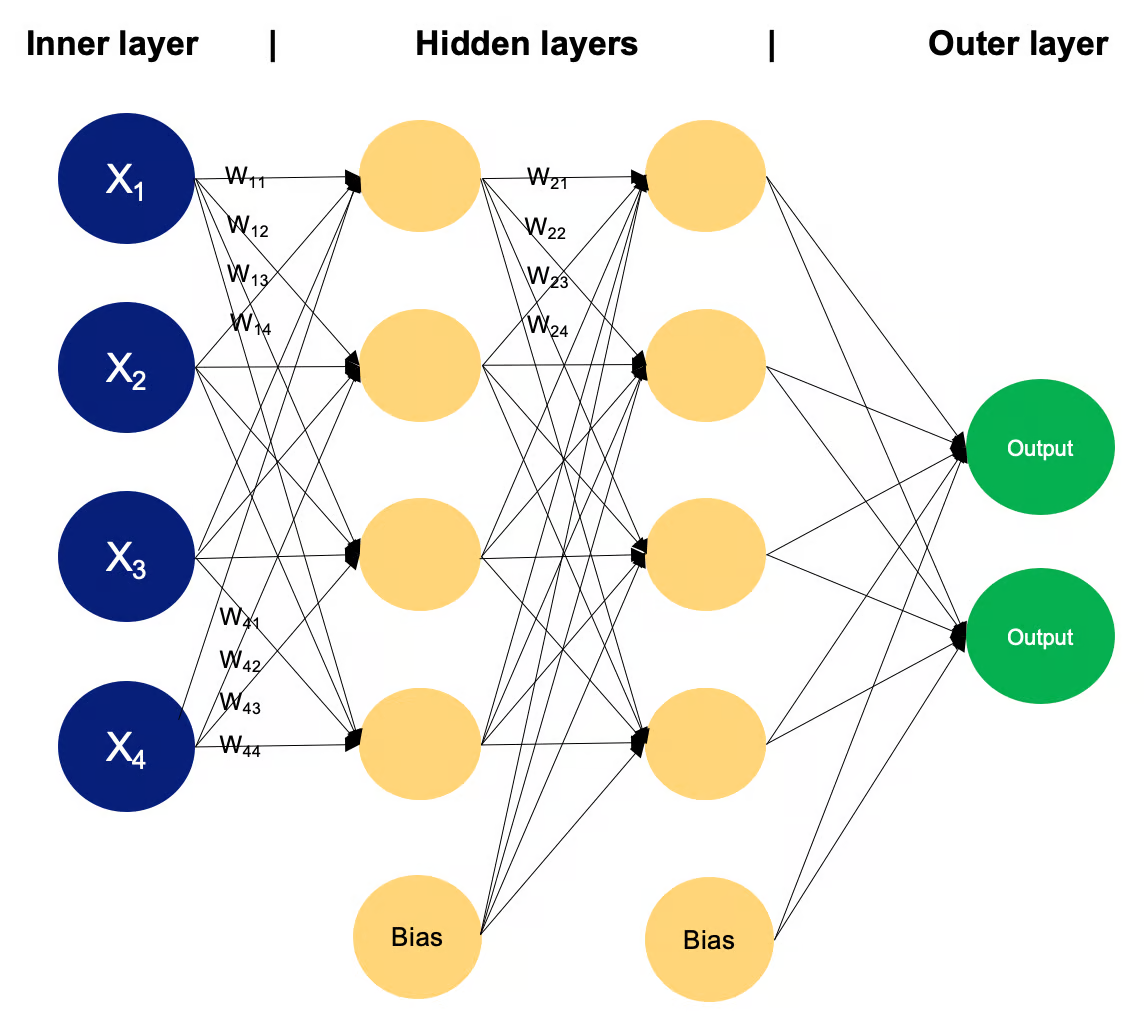
\includegraphics[width=0.7\textwidth]{images/mlp-diagram.png}
    \caption{Basic structure of a Multilayer Perceptron (MLP) \cite{mlp}.}
    \label{fig:mlp}
\end{figure}

In the image, you can observe the flow of information from the input layer through the hidden layers to the output layer. Each layer plays a critical role in transforming the input data to make sense of the patterns and relationships. The neurons in the hidden layers learn features in the data, and as the network adjusts its weights through training, it becomes more accurate in predicting the target outcome.

MLPs are particularly effective in tasks where the relationships between input features and the target variable are non-linear, as is the case in health-related predictions like diabetes classification \cite{deeplearning1}. This model's ability to learn from complex and large datasets allows it to handle a wide variety of problems, from image recognition to medical diagnoses.

What makes MLPs particularly well-suited for our dataset is their capacity to model intricate relationships between multiple features simultaneously. By learning these relationships, MLPs can make accurate predictions, even when the data contains complex, interdependent factors. This makes MLP an ideal choice for predicting the likelihood of diabetes based on a variety of health indicators \cite{mlp}.

\subsubsection{Implementation and Evaluation}

The MLP model was implemented using the \texttt{scikit-learn} library, leveraging two hidden layers with sizes 100 and 50 respectively. The activation function used was ReLU, and stochastic gradient descent was chosen as the optimizer with adaptive learning rate and a maximum of 500 iterations.

Before finalizing the model, we performed hyperparameter tuning using GridSearchCV to identify the best combination of parameters. This ensures that the model generalizes well to unseen data.

\noindent
The best parameters found were:
\begin{quote}
\texttt{\{'mlp\_\_activation': 'relu', 'mlp\_\_alpha': 0.001, 'mlp\_\_hidden\_layer\_sizes': (100, 50), 'mlp\_\_learning\_rate': 'adaptive', 'mlp\_\_max\_iter': 500, 'mlp\_\_solver': 'sgd'\}}
\end{quote}

\lstinputlisting[language=python]{../code/mlp.py}

\begin{figure}[H]
    \centering
    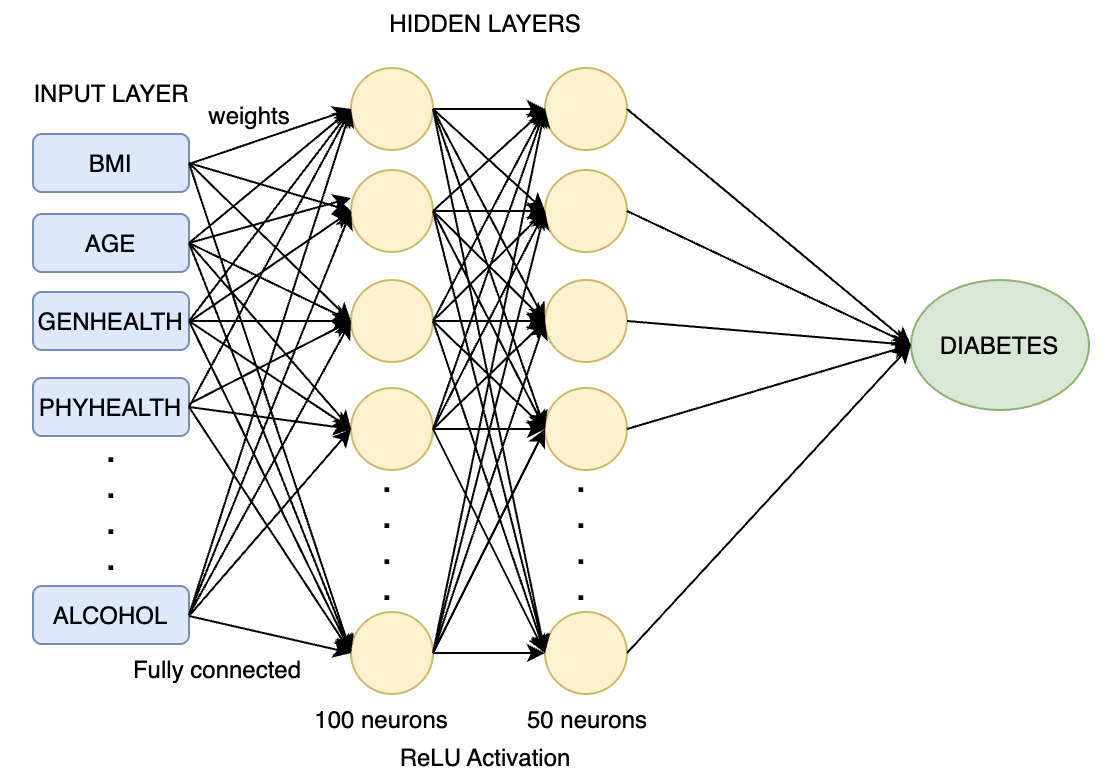
\includegraphics[width=0.75\textwidth]{images/our-mlp-diagram.png} % Make sure the filename matches
    \caption{Our structure of a Multilayer Perceptron (MLP).}
    \label{fig:mlp-arch}
\end{figure}

\vspace{0.5em}

\noindent
Figure~\ref{fig:mlp-arch} illustrates the architecture of the Multilayer Perceptron used in our implementation. It includes an input layer that receives features such as \texttt{BMI}, \texttt{Age}, and \texttt{GenHealth}, followed by two hidden layers with 100 and 50 neurons respectively. These layers apply ReLU activation and are fully connected. The final layer outputs a binary prediction indicating whether the individual is diabetic or not.


\subsubsection{Results on Full Feature Set}

\begin{verbatim}
Performance on Full Feature Set:
Accuracy: 0.7526
Precision: 0.7362
Recall: 0.8011
F1 Score: 0.7673
\end{verbatim}

\noindent
This baseline performance shows that the MLP model handles the full feature set well, achieving over 75\% accuracy and strong recall (80.11\%). Precision and F1-score are also relatively balanced, which means the model is both identifying and distinguishing cases effectively.

\vspace{0.5em}
\noindent
Next, we look at cross-validation results to assess the model’s ability to generalize across different data splits:

\begin{verbatim}
Cross-Validation Mean Scores (5-Fold):
Accuracy: Train = 0.7558, Test = 0.7484
Precision: Train = 0.7359, Test = 0.7295
Recall: Train = 0.8113, Test = 0.8040
F1: Train = 0.7718, Test = 0.7649
\end{verbatim}

\noindent
These results confirm that the model generalizes well, as train and test scores remain consistent across folds. Importantly, test recall remains high (80.40\%), reinforcing the model’s reliability in correctly identifying diabetic cases in unseen data. This cross-validation step validates the single-run results and supports the model’s robustness.

\vspace{0.5em}
\noindent
Now we present the full classification report to explore class-wise performance in more detail:

\begin{verbatim}
Detailed Classification Report (Full Feature Set):
              precision    recall  f1-score   support

 No Diabetes       0.77      0.70      0.74      6753
    Diabetes       0.74      0.80      0.77      7000

    accuracy                           0.75     13753
   macro avg       0.75      0.75      0.75     13753
weighted avg       0.75      0.75      0.75     13753
\end{verbatim}

\begin{figure}[H]
    \centering
    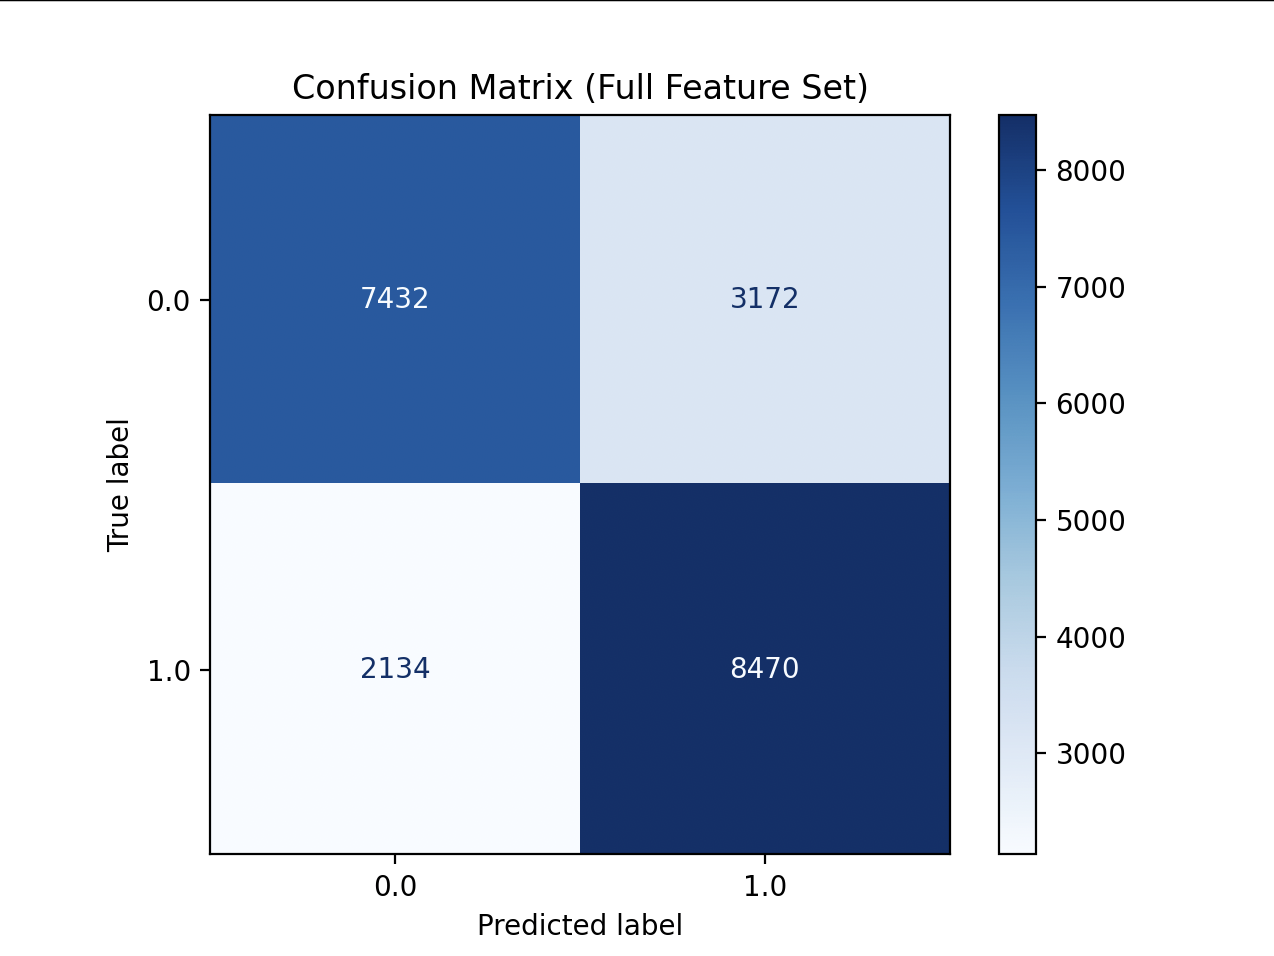
\includegraphics[width=0.5\textwidth]{images/confusion_matrix_full.png}
    \caption{Confusion Matrix for MLP on Full Feature Set}
\end{figure}

\noindent
From this report, it's evident that the model performs slightly better at detecting positive (diabetic) cases than negative ones, with a higher recall for the "Diabetes" class (80\%). This is desirable in our context: it is far more critical to minimize false negatives (undiagnosed diabetic patients) than false positives. Therefore, recall is the metric we prioritize most.

\subsubsection{Results on Selected Features with Interaction Terms}

\begin{verbatim}
Performance on Selected Features + Interactions:
Accuracy: 0.6917
Precision: 0.6633
Recall: 0.8007
F1 Score: 0.7256
\end{verbatim}

\noindent
While accuracy and precision have dropped in this simplified model, recall has remained nearly identical (80.07\%) to the full-feature model. This suggests that the reduced feature set is still effective in identifying diabetic patients, even if it leads to more false positives (lower precision).

\vspace{0.5em}
\noindent
We now show the detailed classification report for this model:

\begin{verbatim}
Detailed Classification Report (Interactions Model):
              precision    recall  f1-score   support

 No Diabetes       0.74      0.58      0.65      6753
    Diabetes       0.66      0.80      0.73      7000

    accuracy                           0.69     13753
   macro avg       0.70      0.69      0.69     13753
weighted avg       0.70      0.69      0.69     13753
\end{verbatim}

\begin{figure}[H]
    \centering
    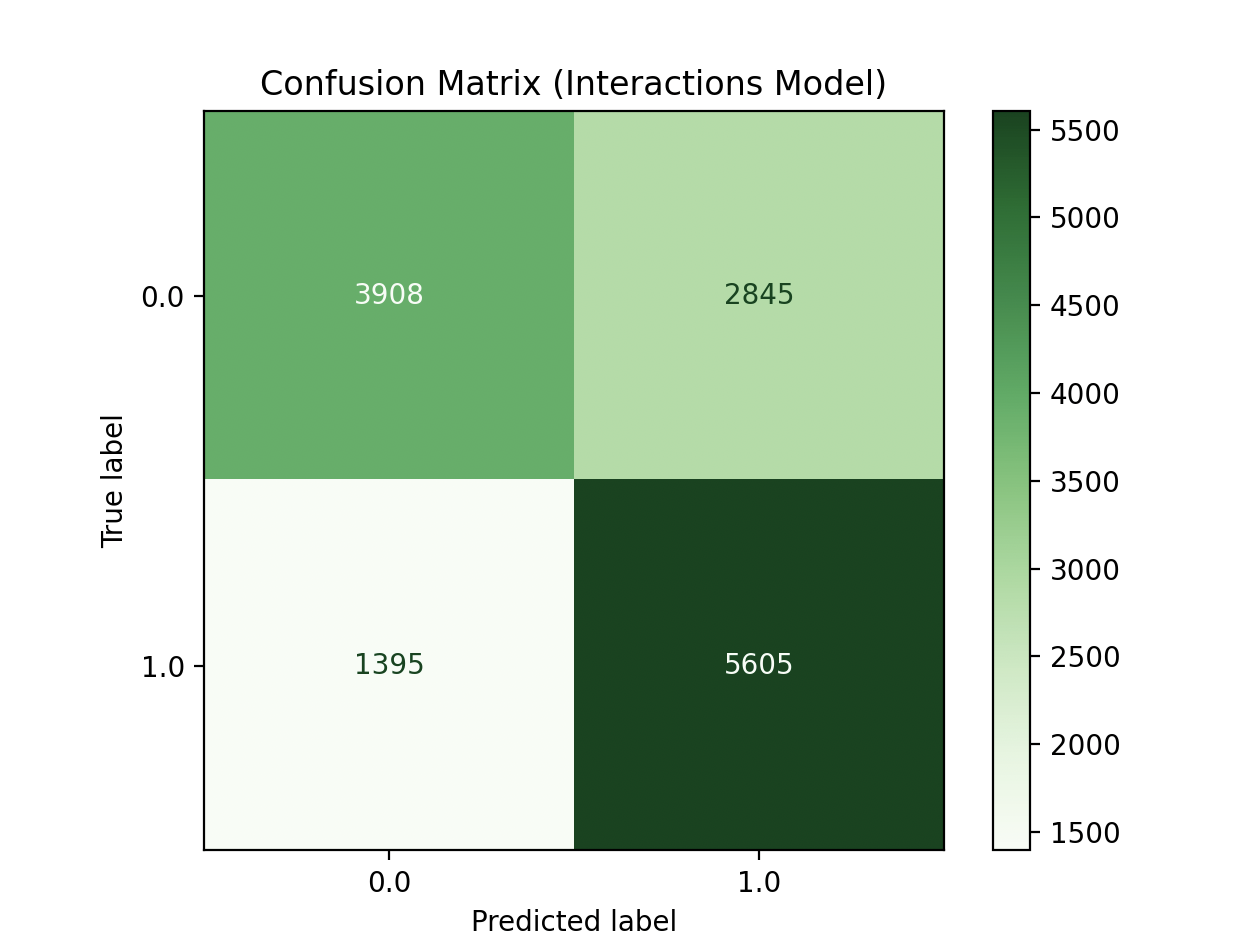
\includegraphics[width=0.5\textwidth]{images/confusion_matrix_interactions.png}
    \caption{Confusion Matrix for MLP on Selected Features + Interaction Terms}
\end{figure}

\noindent
Here again, recall for diabetic cases remains at 80\%, but performance for non-diabetic predictions drops noticeably (recall of 58\%). In practice, this means more people without diabetes are misclassified as diabetic. While this may raise false alarms, it is an acceptable trade-off in medical diagnostics where missing true cases is more dangerous than flagging potential ones.

\vspace{1em}
\noindent
In both models, recall is prioritized above all, aligning with our goal of reducing undiagnosed diabetic cases. The full-feature model is preferred for balanced performance, but the interaction-based model still holds value in more constrained environments.

\begin{figure}[H]
    \centering
    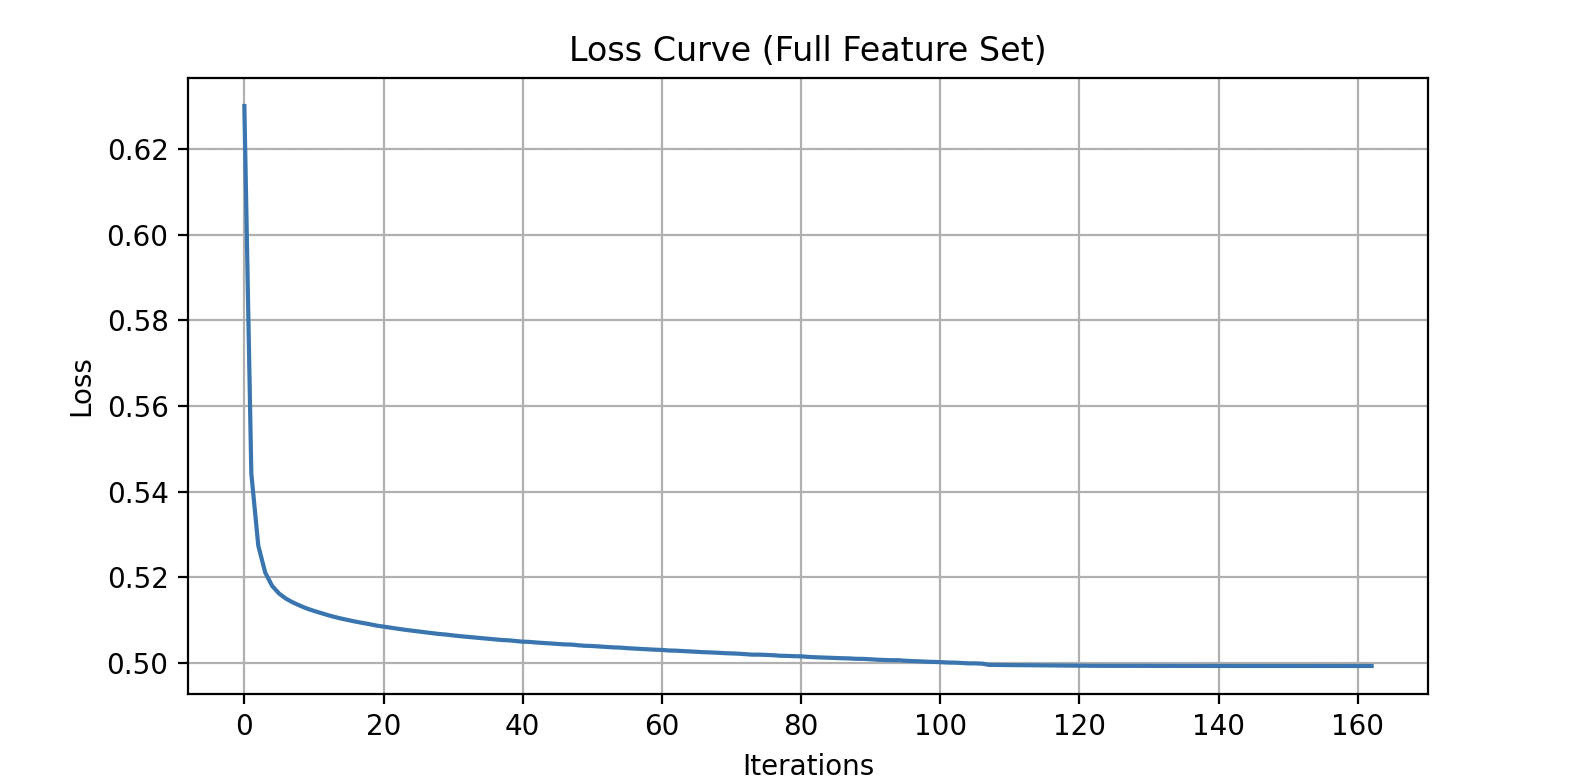
\includegraphics[width=0.6\textwidth]{images/mlp-loss-curve.png} 
    \caption{Training loss curve for the MLP model over 500 iterations.}
    \label{fig:mlp_loss_curve}
    \end{figure}

The loss curve for the diabetes dataset shows a rapid initial decrease followed by convergence, indicating stable training and successful optimization.


\subsection{Autoencoder}

\subsection{Third algorithm}
\section{Result interpretation}

\subsection{Comparison of Algorithms}

In this section, we compare the three applied algorithms—Multilayer Perceptron (MLP), Autoencoder, and Gaussian Naive Bayes—using four key performance metrics: \textbf{Accuracy}, \textbf{Precision}, \textbf{Recall}, and \textbf{F1 Score}. These metrics help us understand each model’s strengths and guide the choice of the most suitable method for our diabetes‐prediction task.

We generally use Accuracy as the default comparison metric since it gives an overall sense of correctness. However, given the medical context, we place extra focus on Recall (to minimize missed diabetic cases) and Precision (to avoid false alarms) as needed.

Before presenting the performance metrics, we reflect on the core questions guiding this study. First, we sought to determine how effectively different machine learning models could predict diabetes risk. The results below compare the three models in terms of their ability to make accurate and meaningful predictions. Second, we investigated whether a limited set of features could generate reliable predictions. In this context, dimensionality reduction through an Autoencoder served to test whether compressed representations of the original features could still preserve predictive power. Similarly, for the Multilayer Perceptron (MLP), we implemented an additional experiment using a reduced feature set, which included manually selected features and their interaction terms. This allowed us to evaluate how feature selection (rather than automated compression) impacts model performance. The following table summarizes how each model performed.
\begin{table}[H]
\centering
\resizebox{\textwidth}{!}{
\begin{tabular}{ |l|l|r|r|r|r| }
\hline
\textbf{Algorithm} & \textbf{Parameters} & \textbf{Accuracy} & \textbf{Precision} & \textbf{Recall} & \textbf{F1 Score} \\
\hline
MLP & hidden\_layers=(100,50), activation=ReLU, solver=SGD & 0.7526 & 0.7362 & 0.8011 & 0.7673 \\
Autoencoder & activation= Leaky ReLU & Sigmoid, opt=Adam & MSE & 0.7400 & 0.7100 & 0.7900 & 0.7500 \\
Gaussian NB & default (GaussianNB) & 0.7381 & 0.7300 & 0.7558 & 0.7427 \\
\hline
\end{tabular}
}
\caption{Performance comparison of MLP, Autoencoder, and Gaussian Naive Bayes}
\label{table:comparison}
\end{table}

In a medical setting, missing a true diabetic case (false negative) is far more critical than issuing a false alarm. Thus, we prioritize models with higher recall. Both MLP and Gaussian NB reach recall levels around 0.80, while the Autoencoder's recall is slightly lower at 0.74.
MLP offers the strongest overall balance (highest F1) thanks to its capacity to learn complex, non‐linear feature interactions. Gaussian NB remains a lightweight baseline with competitive recall and is very fast to train.
An Autoencoder can capture latent structure and reduce noise in the feature space. Even though its overall performance (F1 and recall) is slightly below MLP, it still provides a stable result and is a valuable tool when feature extraction or dimensionality reduction is required.


\subsection{Reasoning}
Among the three models evaluated, the Multilayer Perceptron (MLP) demonstrates the best overall performance, particularly excelling in Recall (0.8011) and F1 Score (0.7673). These metrics are crucial in a medical prediction task like diabetes detection, where identifying true positives is a top priority. While the Autoencoder performs reasonably well and the Gaussian Naive Bayes provides a fast and interpretable solution, the MLP's ability to capture complex patterns and achieve the highest accuracy makes it the most suitable choice for deployment in this context.
\begin{thebibliography}{9}

\bibitem{deeplearning1}
Ian Goodfellow, Yoshua Bengio, and Aaron Courville. 
\textit{Deep Learning}. 
MIT Press, 2016. Available: \url{https://www.deeplearningbook.org}

\bibitem{nn1}
Michael Nielsen. 
\textit{Neural Networks and Deep Learning}. 
2015. Available: \url{http://neuralnetworksanddeeplearning.com}

\bibitem{mlp}
\textit{Multilayer Perceptrons in Machine Learning}.  \url{https://www.datacamp.com/tutorial/multilayer-perceptrons-in-machine-learning}

\bibitem{autoencoder}
\textit{https://hex.tech/blog/autoencoders-for-feature-selection/}
\end{thebibliography}




\noindent\begin{quote}
    \textbf{Tools used:} LaTeX, Python, draw.io, and Google Slides. All code and documentation are available on our \href{https://github.com/eljesa-kqiku/machine-learning-seminar-project}{GitHub page}.
    \end{quote}
    



\end{document}
% \end{document}